\section{Biological Introduction}

\subsection{Tree of Life and the Theory of Life}
The tree of life is both the organizing structure of life sciences (like it's predecessor- Linnean classification) and is a representation of the theory of life - evolution.  On a short time-scale it is a picture of biological reproduction - or unfaithful cloning - a pedigree.  On long time-scales, the tree is a representation of the process of species evolution, which in many ways can be thought of as a pedigree of species, where each node represents a population of a particular specie, and descent down the branches represents time, and division of a node into two nodes (reproduction in a standard pedigree - parents having children..) represents speciation events from a common ancestor (reproduction at a population level on geological time-scales).
\subsubsection{Comparative Anatomy and Physiology}
Previously,in the eighteenth century, Linnean by brute force clustering techniques organized life according to anatomical similarities, leading to a classification system for life. This organization was not just a database that organized collections of living objects by comparative anatomy; the organization explained why the objects were different or why they were similar because comparative anatomy begs the question of 'function', of physiology, and physiology is a theory of life.   In this sense, Linnaen systematic organization of life was a simple theory of life, in that it did explain life, as does all physiology, because it explained the purpose (function) of each anatomical feature\footnote{In biology the 'function' of a trait or anatomical structure is what the trait does or accomplishes, hence the word 'purpose' seems to be a synonym to function.  However, this may be confusing seeing that evolution has no 'purpose', hence 'purpose' should not be interpreted as if the population or lineage that evolved the trait had foresight and intended its creation.}.  For example, the purpose of a leg is locomotion, of a jaw is to bite, of a root is to stabilize a standing plant (among other functions), of a circulatory system (heart) is to circulate nutrients throughout the organism, of a stamen is for sexual reproduction etc.; and Linnaeus knew these trivial relationships between structure and function, which undoubtedly helped in his grouping of organisms.  Interpreting the organization of life through a theory of structure and function is very powerful, as a theory intentionally simplifies complex patterns so that they can be understood and comprehended.  Hence the theory of 'structure and function' has one of the most important aspects of biological theory, and that is to simplify life in a way that we can comprehend its rich diversity.  It also has an obvious predictive power, for example if an animal loses its legs you can predict that it will lose locomotion.  Although many of Linnean groups are based on reproductive anatomical features, a 'structure and function' theory is very short-sighted in terms of how life reproduces, as it can only explain how to maintain existing population of species (by having the reproductive structures do what they do).  What's clearly missing is the origin of life, how to make life from basic physical chemical principles; and the origin of all the different kinds or species once basic life forms (i.e. specie meaning a group that can form viable offspring).

The theory of evolution by Charles Darwin, which I'll summarize in two pieces 'descent' and 'modification' added  more structure to the theory of life.  Darwin recognized (hypothesized) that common anatomical structures were due to common 'descent', indicating common features need not be derived anew possibly using different ingredients each time, the entire structure was passed on during reproduction.  He also recognized that different structures between two groups of animals was due to 'modification' from a common ancestor between the two groups of animals.

\subsubsection{Classical evolution}

Darwin's theory in the late 1800s united life through one common lineage.  However the biological mechanisms of how to produce life from molecules (e.g. how are completely novel and complex features derived in the first place) was not possible during Darwin's time, as the observational tools such as Leeuwenhoek's microscope seemed to be insufficient.  Furthermore to show that one specie of organism could be related to another (through the common ancestor) would require an evolution experiment that takes longer than one's lifetime (usually).  Albeit, as suggested by Darwin's book's title, The Origin of Species, showing that one specie could be related to another was precisely his point.

In parallel with Darwin's work, Mendel's evolution experiment with peas would set in motion the molecular basis of evolution, and set the stage for two contributions from molecular biology that explain the molecular basis of inheritance.  Before the advent of molecular biology, from a reductionist point of view, the proof (evidence) of the evolutionary tree of multicellular organisms can be thought of as a hierarchy of conservation of features or modules.  The importance of conservation can not be stated enough, as Darwin's central tenant is 'descent', meaning common features between our ancestors and ourselves are due to conservation from descent: inheritance.  At the highest level of modularity (and by far the most useful for a big picture resolution of the tree of life for multicellular organisms) is the anatomical structures (e.g. leg, eye, heart, nervous system).  Comparative embryology during Darwin's time elucidated that all these anatomical structures from organs to gross features like a leg (containing multiple organs, like skin) are derived from possibly just three tissue types (germ layers).  For example, the heart is derived from the mesoderm tissue, and all multicellular organisms without a mesoderm in their embryonic stage do not develop a heart.  These three tissue types are composed of largely undifferentiated cells and during development they work together and sometimes work independently to fate the array of different cell types that make up the anatomical features that make up multicellular organisms (such as epidermal cells,  hematopoietic cells, blood cells).  Hence, before molecular biology (before the 'gene' picture), there was at least three basic conserved traits that could be used for evidence on resolving tree branching in multicellular organisms (anatomical features, germ layers, cell types).
    
\subsubsection{Modern Synthesis of evolution}

\textbf{Molecular genetics}, the first contribution from molecular biology, would show animals posses genes that are contained in chromatin and that those genes were passed on from parents to children during reproduction, this culminated in the 'modern synthesis' of evolutionary biology in the early 1900s.  This would gain further support by R. Franklin's crystallization of a chunk of chromatin, DNA.  DNA was found to be a polymer strand that would complement with another self assembling strand, which Francis and Crick saw could serve as a 'copy' for a replicating cell's progeny cell.  The 'modern synthesis' is largely about the molecular dynamics of populations, 'population genetics', a population of organism's genomes (the frequency of genotypes) and how those change in time (in units of generations), and how they can be influenced by natural selection, mutation, gene flow, migration and isolation (E. Mayer type speciation-allopatry).  Most significantly, the gene centred picture that had arisen in evolution now had given a fourth feature or module that was conserved: the gene, which encodes for a protein. 
\subsubsection*{Comparative genomics}
With the advent of fast 'sequencing' technology that can determine the genetic sequence of whole genomes, genetic conservation (by simply comparing genomes) has become a powerful tool in helping resolve the various branches of the evolutionary tree.  With the knowledge of the vast array of processes of genome evolution (how genome's changes in time) we infer the enormous genomes of complex organisms like humans that share genes in common with the much smaller bacterial genomes, share these in common due to inheritance, through the process of natural selection that balances the randomizing forces of mutation, as generation of genes de novo (by random mutation) is far less likely (probabilistically) than the probability of inheriting these modules (genes) (e.g. a gene of length 1000 nucleotide (hence about 333 amino acids) has $4^{1000}=2^{2000} > 10^{300}$ possible sequences, which means an organism that reproduces 1000 times per year would still require vastly more time than the time available since the Big Bang to generate one gene (see J.Maynard Smith's chapter one\cite{maynard}).).  The cause of the genetic inheritance through natural selection can be due to standard reproduction along a lineage (i.e. meiosis and sexual reproduction), such as the human lineage, or it can be due to more exotic forms of homology (inheritance), where viruses or transposable elements can insert genetic material in host genomes resulting in genome expansion, where the newly inserted genetic material may, over time, become a beneficial resource to the host.  Perhaps, the most significant source of genome evolution is gene duplication and whole genome duplication (the human lineage is thought to have had two whole genome duplications since the evolution of the deuterostomes - the 2 rounds (2R) hypothesis\footnote{This 2R hypothesis is supported by whole genome analysis between vertebrates and invertebrates.  In particular the HOX genes as seen on four chromosomes occur on just one chromosome in the fly.}) that can have enormous effects such as those seen in the mustard family of plants.  These duplication events cause each original gene to have a copy whose purpose is in a sense unfated, and hence is free to evolve a new function.  Hence although humans have about 25,000 genes, many of these are just slight variants of one another -a gene family - inherited through duplication events.  Hence, the archibacteria that originated about four billion years ago, evolved gene templates (a basic design) of some of the gene families through natural selection for genes necessary to process the oxygen depleted environment, similarly their descendent cyanobacteria evolved process necessary for photosynthesis, thereby transforming the atmosphere to be amenable for evolution of gene networks in aerobic respiration found in bacteria.  It can then be interpreted that most of our genes (the genes found in eukaryotes) that we share in common with bacteria are inherited from the bacteria.  Hence gene phylogeny has become the standard technique to resolve (determining the branching order) of the tree of life.  Of course, it has been shown that a gene phylogeny almost always agrees with an anatomical grouping (such as Linnaeus groupings), because genes encode the anatomical structures\footnote{One must still be careful using just anatomical features for determining the topology of the tree, as 'mimics' commonly seen in the insect world in predator prey interactions to deceive their opponent clearly demonstrate that anatomical features can be evolved independently\footnote{The mimic's anatomical features are independent of the predator or prey at a genetic level, while they are dependent at an organismal level, where the predator or prey provides the selection pressure to evolve (presumably through co-option of existing genes) the gene's that encode the anatomical features.}.  However, internal anatomy structures like the central nervous system are much stronger anatomical features for determining evolution, since these internal features are very complex and much harder to evolve de novo, and harder to co-opt due to high levels of epistasis and pleiotropy.}.

An obvious question about gene templates (gene families) is how does one infer that a particular gene locus in human (for example) correspond to the same locus in say a fish.  The gene of interest in the two organisms may be the direct descendent in each lineage since the most recent common ancestor of the organisms, or it may be the indirect descendent in each lineage due to gene and genome duplications or viral and transposable element insertions - this is the distinction of orthologs and paralogs\footnote{Convergence indicates the organism generated the feature anew, which is of course a possibility for any material being obeying the laws of physics, but is so much less likely than inheritance that whenever inheritance can be demonstrated possible this is the most probabilistic origin.}.  Of course if the genomes are from a recent common ancestor, like chimp and human, it's relatively easy, since the 'order' of the genes is preserved (synteny), hence the genomes (chromosome) roughly match or align from start to end (barring the five largescale inversions and the famous fusion of two of the chimp's 24 chromosomes forming chromosome 'number 2' in human that has two centromeres and two additional telomeres at the fusion site of the chromosomes, hence humans have 23 chromosomes.).  However, for more distantly related organisms, such as fish and human, this is more difficult due to chromosome inversions and the many indels since the most recent common ancestor.  
\subsubsection*{Expression patterns}
The answer is that we need to know where in the body (where in the anatomy) is the gene being expressed.  If we are interested in a protein in the brain (say $chordin$), we would expect that the homolog (here i use homolog to mean direct common ancestry - so i mean ortholog) of that gene be expressed in the insect brain (say $dpp$).  This expectation is in a sense obvious, as you may know through your own experience with food and taste that different organs and tissue of an animal or plant 'body plan' taste different due to the different proteins in those organs (of course some tissues are full of sugars and lipids possibly overwhelming any taste from the proteins).  If the genes are indeed coexpressed in the same tissue, we next need to know if the gene functions the same way, is its protein being used for the same purpose.  Given that the gene is coexpressed in the same tissue and functions the same, this, by parsimony, would suggest the genes are orthologs rather than paralogs.

How do we see 'where' a gene is expressed in a body (like is it expressed in the brain, heart or muscle etc.)?  This question could be answered partly by classical genetics (breeding using Mendel's laws) by determining if a known genotype resulted in embryonic lethality (or when in development the fetus or larva died, or what environmental pressures would 'induce' death -presumably because of the mutant gene).  However, using classical genetics alone to determine where a gene is expressed in a body is extremely tedious and indirect and has major limitations and requires a lot of interpretation.  A much faster technique would be a visual tag on the gene's protein or mRNA (such as a fluorescent marker or dye), albeit classical genetics is still required to control for the correct allelic version of the gene of interest among other reasons (like genomic background).  This microscopic technology became available in the 1980s and revolutionized are understanding of evolution by using the technology coupled with time-shots of development, thereby also telling us 'when' a gene is expressed during an embryo's development.

\subsubsection{The generalization of the theory of evolution; developmental genetics}
Prior to the 1980s, embryologist and developmental biologist had carefully observed the different stages of development of many multicellular organisms.  Maps were made of the different cell types that would be produced from the single fertilized egg, a cell lineage, as was mapped in detail for the first time in the development of the nematode.  These cell lineages that were derived from the fertilized egg, and then germ layers, would mark the differentiation of cells (or cell specification).  By determining 'where' a gene was expressed in a developing animal embryo it became evident that the process of cell differentiation, was linked with co-expression of whole sets of genes, where at each step of differentiation new sets of genes were being expressed (and other turned off)\footnote{Plant development is different than animals.  Plants ubiquitously display 'phenotypic plasticity', which in development is called 'developmental plasticity'.  Plant development is not a reproducible if the environment of the plant changes (e.g. change the temperature or light and the plant will respond).  Plants respond to their environment, while animals do not, as S.Gilbert puts it: some organisms (like animal development) are ruled by a tyrant genome, where the phenotype plays the passive permissive role of the ruled while other organisms (like plants) are ruled by the environment, where now the genotype plays the passive role of the ruled(see chapter 22 Gilbert\cite{devogilbert}).  Animals have largely evolved plasticity as part of their development, this is a little different than homeostasis.  Hence, 'developmental plasticity' seen in plants is incorporated into animal development.  Animals have stably generated the \textit{internal} environmental cues to turn genes on and off at different anatomical positions of varying molecular environments, where a plant may develop roots if cued by low light levels or various chemical triggers, an animal has put the cues for development as part of its internal system.  For example, animals always develops say a neuroectoderm and mesoderm  because the environmental cues that are a part of the embryonic environment are stable (such as in mother's womb that sets up concentration gradients of key transcription factors, which lead to the Dorsal gradient, or the egg casing of fly or chicken) and are processed by components of the genome (e.g. CRMs)\cite{ecodevo}}.   Hence development in animals, in a large part, can be seen as a result of 'gene regulation'.
 
The second part of molecular biology that supports macroevolution, and possibly an extension of the 'modern synthesis', is \textbf{developmental genetics}. Developmental genetics would show that master genes ( transcription factors) when their regulatory targets or binding sites evolved, then whole developmental networks (i.e. the genes necessary to build an anatomical structure) could be redeployed to a different position of a developing body (e.g. the position that expressed the activator master gene), or lead to modifications of current body parts\footnote{As suggested by the phrase, 'developmental genetics', this would seem to be a sub-discipline of 'molecular genetics' and hence not an extension of the modern synthesis, but rather a refining.  However, the modern synthesis was a gene centred theory; it was about gene's that encode for proteins.  Developmental genetics is a gene 'regulatory' theory, it is about the parts of the genome that turn traditional genes on and off; and gene regulatory elements (transcription factor binding sites) are not really apart of the modern idea of a gene.  A gene encodes for a protein.  A genetic regulatory element encodes for something altogether different.}.  

Developmental genetics to large degree is the field of study that shows at a molecular level how whole anatomical features evolve, and how the diversity of anatomical features and their arrangement (body plans) has evolved.  This is because the detailed molecular mechanisms of how animals develop has revealed the simplicity of anatomical scale evolution (sometimes crudely called 'macroevolution').  Developmental mechanisms are observed in the field of developmental genetics through powerful experiments such as transplantation experiments, and gain and loss of functions experiments, along with the powerful tools of genetics and microscopy techniques.  In a sense developmental genetics, elucidates the 'Gene Reulatory Networks' that form the causal coarse grained molecular basis of self assembling anatomical features. 
\subsection{Development}

\subsubsection{The origin of multicellularity; the evolution \textit{of} development}
About one or two billion years ago, single-celled algae started to cooperate by developing cell cell interactions, forming the first eukaryotic multicellular  organisms, like algal mats.  Such constructs eventually lead to the important innovation of multicellular organisms that is found in animals (and other kingdoms): sexual reproduction through meiosis and fertilization.  Like endosymbiosis, which is possibly the origin of eukaryotes from bacteria, where two cells would merge and partner to share their particular genes and hence traits (which may be different traits), in sexual reproduction cells not only merge, or fertilize (merging of two gametes into a zygote), but they first go through meiosis, which is significantly different from the results of endosymbiosis (which replicate through mitosis of each fused component) significantly different due to the 'recombination' of traits, or crossing over, leading to great diversity in progeny, thereby leading to faster evolution (by Fisher's Fundamental Theorem) and preventing Muller's ratchet (by creating gamete's free of detrimental mutations).  Furthermore, the fusion of two genomes (e.g. the two gamete genomes) is a form of 'gene duplication'.  Genetic duplication events of genes is a source of 'gene families', where the copied gene (paralog) can extend the diversity in function of a particular template gene, which leads to a whole family of genes(a paralog phylogeny, see for example chapter 7 of Durbin et al.\cite{BSA})\footnote{Two bacterial cells could fuse leading to a n $\rightarrow$ 2n genotype, similar to diploidy, and allowing for greater genomic diversity as one of the duplicate copies of the gene are now free to serve a new function.  However, this genome duplication event is distinct from sexual reproduction (and hence is not diploidy, in my opinion), as the new bacteria with 2n genes, can be said to now have simply n' genes (a haploid with n' genes), when the n' genes are replicated (through mitosis), the progeny are clones (if mutation rate is slow enough), which distinguishes it from sex, in sexual reproduction the progeny are not clones due to recombination (assuming the mutation rate is high enough that there exists some genetic polymorphisms in the population, such that the cross over pieces are not identical).}.  

These early sexual reproducing algae are the origin of eukaryotic early development (which I define as eukaryotic cellular interactions that lead to a multicellular structure, such as an algal mat (a plain of cells), or a 'blastula, like the protistan volvox' (a ball of cells)\cite{pmid7579526}).  These primitive organisms are modern representatives and typical examples of the evolution of multicellularity.  

In the diverse domain of eukaryote the most famous groups are multicellular organisms due to their gross anatomical features that capture our attention from due to their beauty and diverse functions.  In the multicellular organisms there is a remarkably conserved early development, yet there is also marked differences in development suggesting that multicellularity has independently evolved in plants, animals, and fungus.  

Examples of multicellular precursors to multicellularity can be even seen in bacteria in quorum sensing (chemical communication/signalling) and the primitive fungus yeast through their form of sex using 'mating types' (mating 'types' are analogs of males and females)\cite{pmid7579526}. An array of protists (eukaryotes that are not animals, plants, or fungus) show multicellularity, notably volvox and slime molds.  All these 'primitive' organisms are good starting points for the study of multicellularity. 

 'Development', to a large degree, focuses on multi-cell types - cellular differentiation (a skin cell 'functions' differently than a germ cell and functions different than a stomach cell that is a digestive cell that can 'eat' absorbed surroundings ).  That is the division of labor through specialized cells, which is not seen in many primitive organisms, rather these simple organisms are displaying 'colonies', which are the aggregates of cells due to mitosis resulting in progeny cells being proximal to one another (which is physically important in development, but it doesn't display the division of the aggregate into different cell types).

The starting point of 'development' is the innovation of meiosis, invented by the protists, and passed on to its progeny lineages of plants, animals, and fungus.  Hence, plants and animals don't derive sex anew for themselves, they were the benefactors of it from a protistan ancestor.  By the union of meiosis with fertilization (the opposite of meiosis, in a sense) the ability to always have an extra copy of a gene, and therefore the ability of a gene to evolve a new function becomes a stable component of life forms (regardless of whether some life forms display a 'haploid dominant' life form, like bryophytes in plants (e.g. moss and liverwort), where the plant one normally sees is the haploid, because most of the bryophytes' \textit{life cycle} exist in the haploid stage).


The great lineages of animals, fungus, and plants all develop from the fertilized 'egg' (the fusion of the two gametes).  'Egg' means oocyte here (one of the gametes) while in the development literature, egg may also mean the structure that encases a baby, like a chicken egg.  Initially in evolution, possibly, there was no distinction between gametes, egg and sperm (technically plants were first so egg and pollen): both gametes were equal in form, just haploid cells, like in yeasts.  Regardless of the controversial origin of meiosis, we see here a clear case of different cell types and an abstract case of the division of labor at the cell level, the emergence of multi-cell types (which, again, is different than simply cell aggregation).  The division of cell types for the first multi-cell type organisms is speculative, but it seems the haploid cell's role in the life cycle of the first meiotic cells was to provide a means to generate unique progeny that were not clones of the parents (through recombination).   

Cell aggregation in the form of colonies or even in the form of complex structures (the rudiments of a body plan) such as seen in the protist volvox or the 'transitional form' between fungus and animals in the choanoflagellates possibly evolved independently of meiosis (which I consider the origin of different cell types).  Cell aggregation is caused by gene products that connect cells together such as cadherins, actin, and microtubles.  Hence one would suspect that the cell adhesion genes would be conserved among the multicellular lineages, however these great multicellular lineages of plants animals and fungus do not conserve some of these genes, such as one of the largest gene families the "receptor tyrosine kinase", and hence they have each evolved development 'from scratch' (by convergence), which suggests that the origin \textit{of} development can not simply be tied into the origin and evolution of body plans (plants have body plans in the form of features like roots, shoots, and leaves; which can be laid out in many ways.  Are plant body plans related to the layout of animal body plans (like head, thorax, and tail)?  For an excellent developmental comparative anatomy between plants and animals see Alberts\cite{Molbiocell}, who shows there is a similarity of germ layers to the fundamental tissues in plants: epidermal cells, ground tissue cells, vascular tissue cells.  Independent evolution of body plans between plants and animals and fungus does not mean we should not bother comparing their different life cycles and body plans or compare their anatomies and physiology.  The potential fact that these great lineages are all independent simply means that the powerful inferences (predictions) that can be made based on common ancestry are not valid (since their common ancestry is irrelevant if each one independently evolved their anatomical structures, hence the only thing constraining their differences would be basic physics and chemistry and the constraints imposed by descending from their common protistan ancestor).  However, their potential multicellular independence is not as independent as some may suggest, there is still the deep homology in that they all still use meiosis and they both must deal with the complexities of transcription in the face of chromatin.  Albeit, homology in meiosis may be of limited help in understanding their origins because plants have a 'cell wall' that is rigid, unlike animal's permeable and agile cell membrane, suggesting that the production of gametes, and the form of the gametes themselves is vastly different between plants and animals (and indeed pollen and how it 'grows' into the female stamen leading to the ovum is very different than sperm fertilizing an egg in animals). 

\subsubsection{Fly Development}

The coarse-grained (in space and time) molecular dynamics of how a fly is self assembled from a maternally laid egg, a single cell, is coarsely understood at the molecular level thanks to developmental genetics.  This does not explain or prove anatomical evolution, however if gain or loss or modification of a master genes (which encode transcription factors acting in early development) or of gene regulatory binding sites that interact with the master genes did result in modification or gain of loss of anatomical features, then this would convincingly explain the evolutionary mechanism of anatomical features\footnote{This type of huge leaps in modification (leaps) of an organism was observed in the fossil record by John Conway (among others), a palaeontologist, which he called the Cambrian Explosion, and is in contrast (contrast does not mean conflict or contradictory) to the ubiquitously accepted 'gradual accumulation' of beneficial mutations that results in adaptations between particular species of organisms (this was even known by plant and animal breeders before Darwin's theory).  The idea of saltation was called 'punctuated equilibrium' by Steven Jay Gould, where periods of gradual accumulation are punctuated by bursts of major anatomical feature novelty.}  

In the 1960s J. Monod and others working with the bacteria \textit{E coli} discovered that transcription factors can influence gene expression by activating or repressing a gene, where the transcription factor itself was activated by environmental cues (such as sugar)\cite{pmid13718526}.  This would mark the start of the field of gene regulation, which would be the central theme in developmental genetics, which was quickly recognized after Monod's discovery by E. Davidson the developmental biologist working in collaboration with a nuclear physicist R. Britain\cite{pmid5160087}.  


In \textit{Drosophila} development it is known that after fertilization of the egg and after cleavage (mitosis without a G phase (cells do not Grow bigger)) within the blastocyst maternally laid transcription factors (such as Bicoid) zygotically regulate other transcription factors (such as gap genes (which are transcription factors) which in turn regulate pair-rule genes (which are transcription factors) which in turn regulate effector genes (like HOX genes, some of which are transcription factors) that ultimately feed in to signalling networks and paracrine factors that lead to the construction of anatomical features.  

The initial maternally laid transcription factors are not ubiquitously expressed throughout the egg chamber, rather, like a Fourier series, the first maternal transcription factor protein forms a coarse pattern across the embryo, where the protein concentration is like a square wave of concentration as a function of space that forms a term in a Fourier series (I mean discrete summation of a few signals).  This transcription factor protein may act alone to activate a gap gene (like \textit{hunchback}) or may act with another maternally laid transcription factor whose pattern is also like a square wave (with a phase shift), thereby \textit{adding} another term to the series.  The addition of the two input signals results after a bit of time in an additional new pattern across the embryo in the form a gap gene's protein concentration.  Hence as time progresses more complex patterns appear as the gap gene's interact (primarily like \textit{addition} of waves in a Fourier series) resulting in patterns like a sine wave (where, again, the amplitude is the amount of protein at a particular time and the horizontal axis is a spatial axis of the embryo (the wave is in space not time), where the embryo's axis length is fixed in time).  Hence, after cleavage in development, the totipotent cells of the blastocyst are in a sense transforming into more specialized cell types, where the cell is defined by the amount of each specific gene product's protein concentration at a particular \textbf{position} of the embryo, where position is emphasized to stress that the concentration patterns are over space (the location of the embryo).  These differentiated cells will divide further and differentiate further as the embryo starts to take the form of an adult segmented fly.  The chain reaction of gene interactions that begins with the maternal transcription factors that activate other transcription factors, which in turn activate other factors, gives a molecular dynamics description of early development, and hence answers the question of how to build 'from scratch' a body plan (the arrangement of anatomical features).  

'From scratch' is misleading and ambiguous when discussing body plans of animals.  There are two issues the phrase needs to invoke, ontogeny (development) and phylogeny (evolution).  Disentangling the ambiguity we see first, how an adult arises from a single fertilized egg using the model system Drosophila.  Second, how did single celled organisms evolve as the diversity of all multicellular organisms.  It is in phylogeny and evolution that the question of how to evolve from scratch an animal is misleading.  Evolution rarely builds from scratch (i.e. independent evolution such as convergence or parallelisms), body plans are thought to derive through the reconstructions of a set of modules (developmental networks of genes) that each encode for anatomical features (hence all eyes, for example, are homologies at a developmental level through the master gene (transcription factor) \textit{pax6} that binds to a set of genes that set a 'totipotent' or partially programmed cell to start to 'develop' the eye imaginal disc (the set of cells that form the basic outline of an eye, which when induced, will form an eye (at any part of a body that 'induction' occurs (even in the tail region if so induced)\cite{devogilbert}.  

The ideas of a totipotent cell and cell specification are necessary to explain development, and hence necessary component of an extension to the modern synthesis.  I will briefly discuss cell differentiation and cell lineages below in the origin of multicellularity.  Of course, the initial body with many of the modules (urbilateria, the ancestor of all animals) or its fungal ancestor, still needs to be explained as how one builds it from scratch ( this is being done using choanoflagellites and brine shrimp -artemia), but most people are satisfied making inferences with a hypothetical urbilateria that can explain the diversity of animals by the evolution of gene regulatory networks.  Furthermore, the statement that anatomical features are modular at the genetic level is not obvious, as many believe complex features (anatomical structures) contain highly correlated genetic networks, such that any genetic mutation would be deleterious and probably lethal.  The discovery of the extent of modularity (or the extent of nonmodularity through 'induction' by signalling and paracrine factors) I will discuss briefly in the section below on 'modularity'.        
%\subsubsection{Comparative Embryology}


\subsubsection{The crowning jewel of Evo-Devo: the HOX genes}
The work of Ed Lewis (a PhD student of Alfred Sturtevant) on body-transformative genes that were 'saltationary'\footnote{Saltation is the idea that within just one generation major evolutionary transformations could occur, possibly even speciation, taking the idea to its fictional extreme would be like an ape having a baby human, a 'hopeful monster', hence in one generation a speciation event occurred.  Of course this example uses the least derived (the organism with the fewest features) as the poster child for the ancestor (e.g. algea for protist, sponge for monoblasts, jellyfish for dipoblasts, worms (like nematode) for tripoblasts, ape for Hominoidea...)} helped provide evidence and a theoretical framework (extending evolution theory) for the statement that diversity in the animal kingdom (in particular the \textit{segmented} insects) is due to evolution of gene reguatory networks.  The "Hox" genes were a group of genes that caused 'Homeotic transformations', which means a transformation in a body part of an animal 'into' another part, like changing a pair of legs into a pair of antennae.  These mutant transformations that were known to some biologist such as Bateson (who also coined the word 'genetics') as early as the late nineteenth century, who had catalogued these in various animal groups such as crabs and flys etc..  An exemplary gene in the HOX group is 'bithorax', which was discovered in Thomas Hunt Morgan's fly lab around 1915, and a lineage of these mutants has been preserved since then. The gene is named after its mutation that lead to a mutant fly with two (bi) thoraxes (like an abdomen).  Lewis found that further crosses with other mutant lineages lead to double the number of wings of the fly (since the thorax is where the wing's developmental source (or pool of cells that each have the right genes turned on and off- a form of programming - leads to the developmental source of cells of the wing, these 'programmed' cells during early development are the so-called 'imaginal disc', and in this case, the wing imaginal disk\footnote{place a 'wing imaginal disc' in the location of the head, and you get wings growing out of the head, or place a 'leg imaginal disc' - the cells 'programmed' to build a leg where a wing is supposed to occur and you'll see leg's 'grow' or further develop where the wing's were supposed to be.} occurs, and hence is a homeotic transformation.  The Morgan lab didn't know the molecular genetic basis behind bithorax (what DNA sequence had changed (or possibly networks of DNA sequences) from the wild type fly to the mutant), but they did know the mutation was inheritable, and hence was genetic.  They also were able to 'map' the location of these genes (before they even knew genes were made of DNA) to locations on the chromosome due to a technique developed by Morgan's undergrad student (Alfred Sturtevant), who had inferred that genes must be linearly arrayed along the chromosome, which would suggest 'linked' genes (or linearly close genes along the chromosome) would not recombine that frequently during meiosis\cite{sturtevant}.  

Armed with the knowledge of the location of the genes that contributed to the so-called bithorax complex (due to Sturtevant's mapping technology), Lewis created a model of how the bithorax HOX genes evolved from an ancestral gene through tandem gene duplications (which is largely thought correct) which culminated in his theoretical paper in 1978\cite{pmid103000}.  Lewis knew through his own genetic gain and loss of function assays the behavior of HOX genes when crossed with various mutant fly lineages (due to classical genetics Lewis could create hybrid flies due to recombination during meiosis to create crosses of known mutant HOX lineages of flies, such as bithorax line).  From these experiments he constructed a Wolpert-like gradient model (e g. French Flag Model) of how the HOX genes would interact like a Fourier series, one HOX gene would be coarsly expressed, thereby turning on another HOX gene in the complex, then the two of these would work in tandem to turn on a third HOX gene, then the three would all work in unison to turn on the fourth HOX gene.  Central to his hypothesis was not just the consecutive combinations of the HOX gene products activate new HOX genes in the complex, but also that each new actively generated HOX gene would repress the most recent in time activated gene, thereby creating fine patterns of gene expressions within the cells of the embryo.  These unique gene products across the embryo were isolated in segments in space (he could literally see the segments, as these were gross anatomical features each containing 1000's of cells in early development).  

Hence, Lewis had proposed a developmental mechanism for how each segment contained different sets of gene products, and thereby explained how each segment would set in motion the signalling and paracrine factors that would eventually cause the segment to form an anatomical feature like a leg, wing, head, or tail.  The HOX genes are transcription factors (master genes) that target the genes necessary in signalling pathways and paracrine induction.   In short, Lewis had a hypothesis for how anatomical features were built from the segmented larva, but more importantly, he saw an evolutionary mechanism for saltation or macroevolution by his model of the HOX genes; as the basis of HOX genes is that if you mutate them, then the segments of the fly would change in such a way to suggest that the anatomical features that decorate the segments (antennae, wings, legs, eye, abdomen etc..) were all just one ancestral anatomical feature like a leg for locomotion, that could be adapted or modified for further purposes, like an antennae for sensing the environment, or a mandible or claw for killing prey.

It is now known that there are just three HOX genes in the bithorax complex.  While, Lewis had proposed more than this because of various mutations in different locations of the same gene.  The HOX genes display various splice sites, and various gene regulatory elements, where mutations in a particular exon or particular transcription factor binding site would cause different phenotypes.  Although Lewis didn't get everything right, to a large degree he had proposed correctly one of the greatest theories of biology, how genes 'regulate' development (by master genes turning on other genes necessary for building the anatomical features), and how these genes, when mutated, can lead to major rearrangements of anatomical features. 

The question of how the segmented larva developed from the fertilized egg was being elucidated in parallel with Lewis' work through experiments of early development to identify genes involved in forming the fly's body structure.  Partly through the extensive genetic mutation experiments of Christiane Nullsein Volhard and Eric Wieschous that identified embryonic lethal mutants (and therefore gene's active in development) it became clearer that there were maternal laid and zygotic genes (transcription factors) that caused Anterior Posterior segmentation in the larva from the humble beginning of the fertilized egg, these genes are known as the gap genes and the pair-rule genes due to the mutant patterns that the would cause in the early embryo and larva\cite{pmid6776413}.  

Although a genetic description was emerging of how the fly develops, it was not possible to isolate the gene products of flies at tissue specific locations at the time of Wieschaus, Nusslein Volhard, and Lewis due to the gene's protein being inside of a multicellular environment\footnote{For example, Lewis knew the locations on the chromosome of what gene's caused homeotic mutations, and what segments of a larva were effected by the mutation; but Lewis simply didn't know to what extent that gene's product caused the mutation (it obviously could have been through some convoluted web of interactions).}.  However, primitive techniques for isolating genes was becoming developed due to recombinant technology being produced thanks largely to the discovery of bacterial enzymes that could cut and paste genes from chromosome segments (which is part of bacteria's primitive immune system).  Allowing for foreign DNA to be designed and inserted in bacteria to create vast amounts by simply allowing the bacteria to  divide (to grow colonies) - genetic cloning. In addition FISH, flourescent \textit{in situ} hybridization was being reconginzed as a method to isolate genes through cDNA.
 
  Work by McGinnis and Levine in Walter Gehring's lab and others, in the early 1980s, possibly motivated by Lewis's hypothesis that \textbf{all} the HOX genes are paralogs, lead to the development of a molecular optical \textit{in situ} hybridization technique that allowed one to visually confirm and isolate the region (tissue specific) of expression of each HOX gene in specific segments of the fly, where they wanted to know whether a HOX gene like \textit{antennapedia} was really just expressed in the head (where the antennae appear).  As Lewis had hypothesized, every HOX gene were almost identical (they were paralogs), all of which contained a DNA binding domain called the homeobox, a stretch of about 60 amino acids that encodes the binding domain\cite{pmid6323992}.

A combination of the new microscopic technique, along with genomic sequencing, and bioinformatic pattern recognition techniques has now allowed for developmental biology to quickly advance by elucidating each gene expressed in each cell, and if that gene's product is a transcription factor, where that gene binds within the genome to determine the targets of the factor.

 

\subsubsection{Evolution of body plans in animals}

The diversity of the animal kingdom cannot be explained by standard gene molecular evolution (evolution of gene's encoding proteins); the differences between proteins in animals is not sufficient to explain the diversity in animal phenotypes\cite{pmid1090005}.  It is thought there is about 25,000 proteins, and these proteins (for example, hemoglobin) are largely conserved across the entire kingdom.  The diversity is now thought, to a large extent, to be due to the way these proteins are used in different amounts and in different combinations in different cells and body parts of different multicellular organism.  To change the amount or create combinations of various proteins in a particular cell in an organism is accomplished by gene regulation, along with expansion of genome sizes (from the early bacterial and protist) through gene duplication allowing the roughly \textit{same} protein to adapt to a new niche in the organism.  Hence, in short, the diversity is due to the evolution of the elements of gene regulatory networks, where the transcription factor binding site is THE fundamental unit.

 

\subsection{Gene regulation}

  
\subsubsection{Conserved Gene Regulatory Networks}
	Similar to predictive power of theoretical physics, where general laws have been developed (sometimes over centuries of work) to describe and explain matter; in biology the general theory is evolution.  Unfortunately, evolution only provides predictive power (in terms of comparison) when genetic inheritance governs a particular group of species.  A major aim of biology is to understand what elements of biological systems are conserved between distantly related organsims.  This is because one can then interpolate that all the organisms derived since the last common ancestor of the organims have these features in common.  Therein lies the powerful predictions found in biology.  The prediction that not only are the few sparse observations descriptive of the data, but that it also provides information about all of the unobserved organisms since the last common ancestor of the data.  Hence, in development a major aim is to understand what gene regulatory networks are conserved, thereby providing laws and rules of regulatory networks that are not just confined to a particular model organism, but entire clades.  A number of gene regulatory networks have been shown to be conserved, along with particular strategies in terms of circuit types (e.g. feed forward circuit).  Briefly, I will review two major themes in gene regulatory networks (axis polarity and patterning) and their extent of conservation.
\subsubsection{Anterior Posterior (AP) axis formation}
AP HOX genes are conserved.  However the maternal element Bicoid is derived, which seems contradictory to the idea that for master genes the earlier they are turned on in development the more effect they will have on downstream components of developmental pathways.  The Bicoid protein gradient is formed during oogenesis (the maternal process of producing the unfertilized egg), where maternally laid mRNA becomes localized to the anterior portion of the egg casing.  The egg casing is a multicellular structure that upon completion of oogenesis all of its cells but one (the egg) dissipate and form part of the yolk surrounding the egg's nuclei, all of which is inside the egg casing\footnote{I'm considering the 'nurse' and 'follicle' cells as a part of what I'm calling the 'egg casing'.}.

Master genes such as Bicoid are usually thought to be highly pleiotropic (form network hubs) in that they causally interact with many target genes (which in turn will interact with further genes).  The fact that Bicoid is not a conserved element of development across the animal kingdom suggests that even the upstream elements of developmental pathways are modular (can be substituted) or that there are multiple ways (paths) that lead to the same developmental outcome.

Although Bicoid is not conserved, some of the downstream elements of AP developmental pathway are conserved most notably the HOX genes ,which have been shown to be present even in chordates (which includes the vertebrates, and some weird invertebrates like echinoderms).  The conservation of the HOX genes in mammals and insects was confirmed not only by sequence similarity (i.e., homeobox sequence conservation), but also in that the HOX genes expression patterns are similar during development and play the same functional role in laying out the location of the anatomical features such as head and tail.  Indicating that the genetic instructions for how the embryo 'knows' where to form the body structures is an ancient conserved network that has been so useful to the animal kingdom that it has been preserved since the Cambrian explosion\footnote{Using the construction of a home from a master builder (maybe an architect) as a metaphor, the master genes (i.e. the HOX genes) don't tell the developmental program 'how' to build a wing, it tells the program 'where' to put the wing in the home.  Hence 'master builder' is a bit misleading of a metaphor, they don't build anything, they simply give crude locational cues of where certain features should begin to be built.}.  One of the seminal experiment that confirmed the genetic role of the genes that shape body plans in the animal kingdom was with \textit{eyeless} and \textit{pax6} in 1994 in Walter Gehring's lab\cite{pmid7914031}, where an insect's gene early in development that is known to cause loss of compound eye formation (\textit{eyeless}) was replaced by a similar gene found in mouse (which controls where the mouse eye forms, which is a different form than the fly's compound eye).  Using molecular biology techniques the endogenous insect gene was replaced with the mouse gene, where it was found that the fly still formed compound eyes using the mouse gene, suggesting that the \textit{eyeless} gene is ancient gene that instructs the embryo to form an eye.  What kind of eye?  That is not a question answered in body plan genes.  The developmental genes necessary to instruct the embryo where each anatomical feature goes (the master genes) are fundamentally distinct from the genes that actually are critical components of the actually anatomical structure.  For example, the gene \textit{eyeless} is found (expressed) during the development of the eye (i.e., it is expressed during development in locations of the embryo where an eye will form), but it is not found (not expressed) in the fully functional eye (the adult structure).  Hence, the body plan genes are similar to bankers or stock brokers in a financial system, who don't actually produce any tangible products like music or a cup of coffee, rather they help set in motion the complicated web of interactions that can bring these commodities together in a harmonious manner\footnote{Some HOX genes, like \textit{dpp}, are master genes that play the role of putting disparate object together in harmony, but they also play other roles latter in development, such as in the literal construction of body parts (such as the nervous system for \textit{dpp}).}. 

Further evidence of this significance was corroborated by modifying the expression pattern of this gene (ectopic expression), which would cause eyes to form at different locations of the body\cite{pmid10461206}.  Hence, the HOX genes are all examples of master genes (transcription factors) whose role is in regulating how the animal is to build itself into the fixed arrangement of body parts that help define each animal specie. 

\subsubsection{Dorsal Ventral (DV) axis formation}
The early steps necessary in forming the Dorsal Ventral axis of the fly embryo, much like the AP network, are set in motion during oogenesis, where in the case of DV, at the same time the Bicoid mRNA is producing a gradient in the unfertilized egg, in parallel a gene called Gurken (which is transcribed from the egg's nucleus, unlike Bicoid, where the mRNA were maternal) polarizes the DV axis of the encasing egg by localizing to one side of the future embryo (this side becomes the 'end' of the Dorsal axis, and directly opposite of this side becomes the Ventral side of the future embryo.  Shortly after Gurken localization and DV axis polarization, a maternal gradient of Spatzel is created from a series of protein complex degradations or splits induces the 'Toll pathway', an ancient pathway conserved between humans and bacteria used in innate immunity, where Spatzel binds to the Toll transmembrane receptors that signal to a maternal complex of Cactus and Dorsal protein that in turn causes the complex to split and the protein Dorsal now displays a nuclear localization signal, that allows it passage into nuclie, where Dorsal acts as a transcription factor.  Hence the more Spatzel the more Dorsal that is unlocked from the complex, leading to a Dorsal nuclear concentration gradient that mirrors the Spatzel gradient. Dorsal acts as a transcription factor (hence Dorsal is a master gene).  For example, in early development Dorsal targets a number of genes actively turned on and turned off in the neurogenic ectoderm as shown in figure \ref{shift2}.  Unlike most master genes, Dorsal in turn is activated by a signalling network (not other upstream master genes).  Furthermore, Dorsal interacts in early development with \textit{cactus} a 'maternal effect genes', a set of genes discovered by Nusslein-Volhard and Anderson in 1984, where the initial egg's Cactus protein is transcribed from maternally laid mRNA \textit{cactus} maternal genes.

  Dorsal acts as a coarse grained regulator of the DV axis by forming roughly three different cell types from the totipotent blastula.
  
\begin{figure},
  % Requires \usepackage{graphicx}
  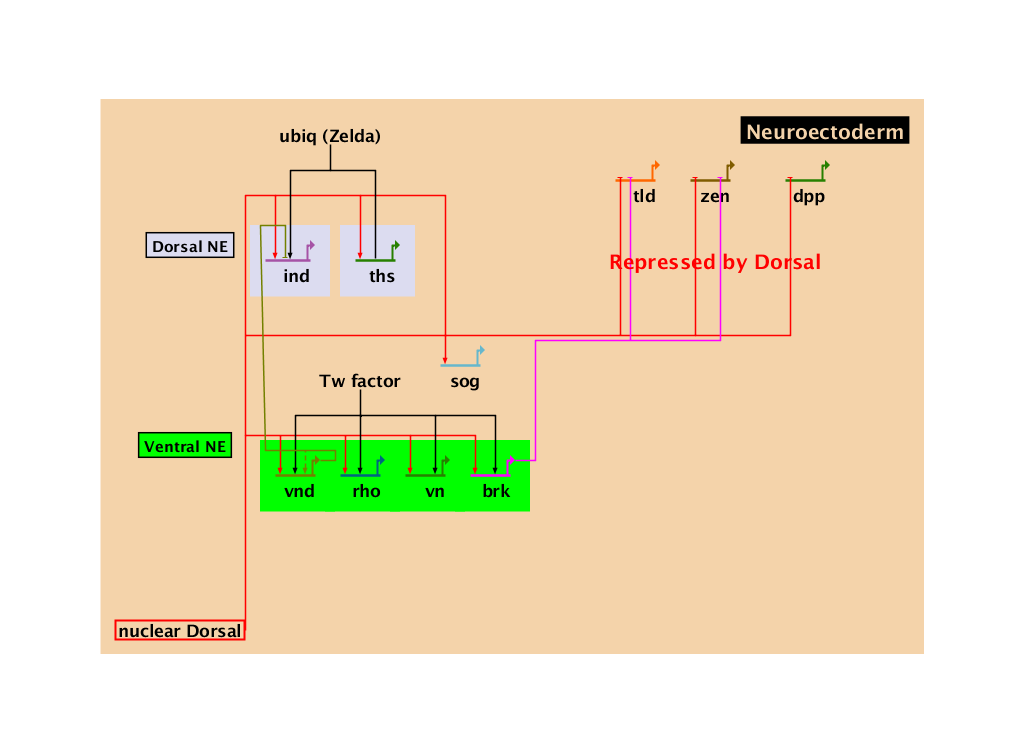
\includegraphics[width=1\textwidth]{slide2jacob}\\
  \caption{Circuit diagram of Dorsal gene regulatory network in the neuroectoderm tissue of early development designed using Angela Strathopolis' template at the Marine Biology Laboratory's Gene Regulatory Networks summer course.}\label{shift2}
\end{figure}
  
  
    These three cell types are components of the 'germ layers' (three primitive tissues seen in all 'tripoblasts' - the animals with bilaterial symmetry that have both a mouth and anus (i.e. go through gastrulation).  Dorsal helps form the mesoderm, neuro-ectoderm and dorsal-ectoderm; where the endoderm is partly constructed by AP genes.  The endoderm is the first evolved germ layer that distinguished inside from outside of primitive 'diploblastic' organisms; animals with radial symmetry like echinoderms that only have one hole (no gastrulation) that serves as both a mouth and an anus (like jellyfish)), where the ectoderm served as the 'outside' of these primitive organisms (hence the mesoderm and the 'triploblast' clade are a more recent evolutionary invention than the 'diploblasts'). 

% The time point of development where Dorsal begins to act like a master gene (a transcription factor) is same point in time when Bicoid is causing its targets to become expressed.  How is it that each developmental pathway DV and AP is simultaneously operating in a given cell of the embryo?  The modularity of the transcription factor binding sites allows for AP target genes to only have DNA binding sites for Bicoid, and similarly DV target genes to only have DNA binding sites for Dorsal.  Similarly as Bicoid works in tandem with some of the genes that it activates (such as Hunchback and Giant), these AP transcription factors combinatorial act together by binding to their target sites that co-occur in short segments of DNA (about 300 bp) that are near the target gene.  By excluding Dorsal and other DV master transcription factor binding sites from these CRMs, AP developmental pathway can proceed in a particular cell in the embryo independently of the DV developmental pathway that is also operating in that same cell.

Just as Bicoid is a derived feature in flys, similarly Dorsal's use as master gene in fly is a derived feature.  The seminal experiment of DV axis polarization in chordates was through experiments by Spemann and Mangold that revealed the source of the germ layers was localized to one side of the vertebrate embryo (they used translucent newt embryos), which was discovered by Spemann artificially splitting the embryos in half by putting a thin belt of string around the tiny embryo and squeezing the string tight, in a way acting like the contractile ring of cytokinesis\cite{devogilbert}.  Their famous transplantation experiment revealed that the analog of the fly's germ layers constructed from the Dorsal transcription factor's gradient, where Dorsal binds to CRMs of DV target genes, was occurring in a small localized region of the newt embryo (completely different that insects).  Spemann called this region the 'organizer'.  What Spemann had discovered was that to a large degree, vertebrate embryos are almost entirely yolk in early development.  And in early development, the embryo forms in a very small region of the 'egg', the organizer, where the majority of the peripheral region of the egg is just 'yolk', which supplies necessary molecules and energy late in development inside the egg.   

Although there is no homolog of Dorsal active in early vertebrate development, the targets of Dorsal found in fly, are also found active in vertebrates.  Twist and Snail are found active in the mesoderm (the Spemann Organizer) and most famous is \textit{dpp} and \textit{sog}, where their homologs form an antagonistic gradient in vertebrates that patterns the notochord (albeit in chordates there has been an 'inversion', which, for example, leads to hearts being ventral in vertebrates while dorsal in most invertebrates).  The notochord is a derived vertebrate feature that forms just below the neural tube ( the future brain and central nervous system that becomes decorated by the vertebra)\footnote{Tunicates develop a gelatinous notochord in early development, suggesting these primitive sea organisms are closer to humans than flys are! showing not all paths of evolution lead to complexity.}. 

The fact that Dorsal is not found to be the master gene that patterns the vertebrate organizer (the germ layers) is very perplexing, just as confusing as why Bicoid is not found upstream of the developmental pathway that leads to activation of the HOX genes in vertebrates.  Furthermore, vertebrate development, to a large degree, seems very different than the localization of transcription factors to specific regions of the embryo (protein gradients), where the different germ layers emerge at specific locations in space due to the various interactions of the protein (morphogen) gradients. Vertebrates use 'induction' (cell-cell interactions) early on in development as a patterning mechanism, where, for example, the endoderm is first formed by the organizer, juxtaposed against a somewhat undifferentiated layer of cells (Nieuwkoop center), where the endoderm - Nieuwkoop interaction in turn induces the formation of mesoderm tissue.  Hence, unlike in flys, where all three layers form somewhat simultaneously, in vertebrates the endoderm forms first, which in turn induces the development of the mesoderm (albeit, the mesoderm targets of Dorsal in fruit fly are activated first, where Snail's expression border helps differentiate neuroectoderm tissue from mesodermal tissue). 

  Perhaps these master genes (Bicoid and Dorsal) are a modification of mitosis' chromosome separation, which became fixed in some of the insect lineage.  In mitosis the microtubles attach to centromeres to direct the movement of the duplicated chromosomes during nuclear division, while in oogenesis the actin attaches to Bicoid or Gurken mRNA leading to dynesin or myosin motors moving these mRNA transcripts to localized region of the egg.  Perhaps the radical differences in insects and vertebrates suggests that urbilateria never existed; that the protostomes and deuterostomes independently evolved from a unicellular protist, albeit, the conservation of the HOX genes would seem to rule this out.  Regardless, by strategically choosing organisms (transitional forms) in between vertebrates and invertebrates these questions can begin to be answered by looking at how, for example, the regulatory regions of \textit{dpp} and \textit{sog} have evolved to be inserted in the developmental pathway of organsims in the vertebrate lineage.  An 'insertion' event of \textit{dpp} and \textit{sog} in vertebrate genomes is not accurate, as the genes are conserved between invertebrates and vertebrates, rather the binding sites of the factors that regulate \textit{dpp} and \textit{sog} must have evolved to respond to the particular factors active in the respective lineages, the evolution of these binding sites is what would help reveal the origin of the event that led \textit{dpp} and \textit{sog} to be regulated by different activators in early DV patterning.
%\subsubsection{Multiple Sequence Alignment}
%Conservation of genetic elements (conserved DNA sequences) is the basis of similarities in Linnean groups, in species.  Mutation of genetic elements is the basis of difference in species.  Conservation of genetic elements is as simple as comparing to words (sequences) by checking if they 'match' at each position.

\subsubsection{Modularity in gene regulatory networks}

 The time point of development where Dorsal begins to act like a master gene (a transcription factor) is the same point in time when Bicoid is causing its targets to become expressed.  How is it that each developmental pathway for axis specification (DV and AP) is simultaneously operating in a given cell of the embryo?  The modularity of the transcription factor binding sites allows for AP target genes to only have DNA binding sites for Bicoid, and similarly DV target genes to only have DNA binding sites for Dorsal.  Similarly as Bicoid works in tandem with some of the genes that it activated in the first place (such as Hunchback and Giant) in feedforward circuits, where these AP transcription factors combinatorial act together by binding to their target DNA binding sites that co-occur in short segments of DNA (about 300 bp the \textit{cis} regulatory modules (CRMs)) that are near the target gene.  By excluding Dorsal and other DV master transcription factor binding sites from these CRMs, AP developmental pathway can proceed in a particular cell in the embryo independently of the DV developmental pathway that is also operating in that same cell.  Hence, these circuits, or components of the developmental pathways that are 'patterning' the embryo (fating the cells through cellular differentiation) are modular.  Late in development, once the nervous system has grown, the modularity seen in laying out the body plan that has organized the anatomical features largely disappears, as the body becomes an integrated system highly interdependent and controlled by the nervous system.
%\subsubsection{\textit{cis} regulatory modules}

\subsubsection{Transcription factor binding sites}
Gene regulation occurs at various temporal and spatial levels.  Within a cell, the amount of a particular protein can be regulated at 'translation' level by regulating the amount of mRNA transcripts that are translated.  However, transcription is the process that is predominantly regulated during development.  

At the finest spatial level, transcription factor binding sites provide the docking area for transcription factors to temporarily bind and in various ways modify the transcription of nearby genes.  The binding process physically depends on the concentration of the transcription factor and the number of binding sites that reside within a CRM.  The flanking sequence of a CRM acts as a competing location for the binding of the transcription factor, hence knowing the size of a genome (i.e. the number of flanking binding sites) is equivalent to knowing the chemical potential.  Thermodynamically a transcription factor follows the chemical potential gradient, hence unoccupied sites in the genome compete for binding of a given transcription factor.  

CRMs have evolved strategies to recruit transcription factors by creating highly specific binding sites that reside within the CRM.  These very specific binding sites provide a potential energy 'well' that captures transcription factor due to the very low binding energy of the well (compared to the high energy of docking at the flanking sequence of the CRM).  Furthermore 'binding cooperativity' also provides a further drop of the potential well for a given transcription factor if a particular cooperating factor is bound nearby.  

